\section{Bundle Protocol Version 7}
\label{penning2019dtn7:sec:bp7}

This section gives an overview of bundle protocols, referring to RFC 4838~\cite{rfc4838} and the current version of the Bundle Protocol (BP) ~\cite{dtn_bp7v13}. The latter has version number 7 and is currently still in active development. We discuss the status of the 13th draft from April 2019 below.

\begin{figure}[tbph]
    \centering
    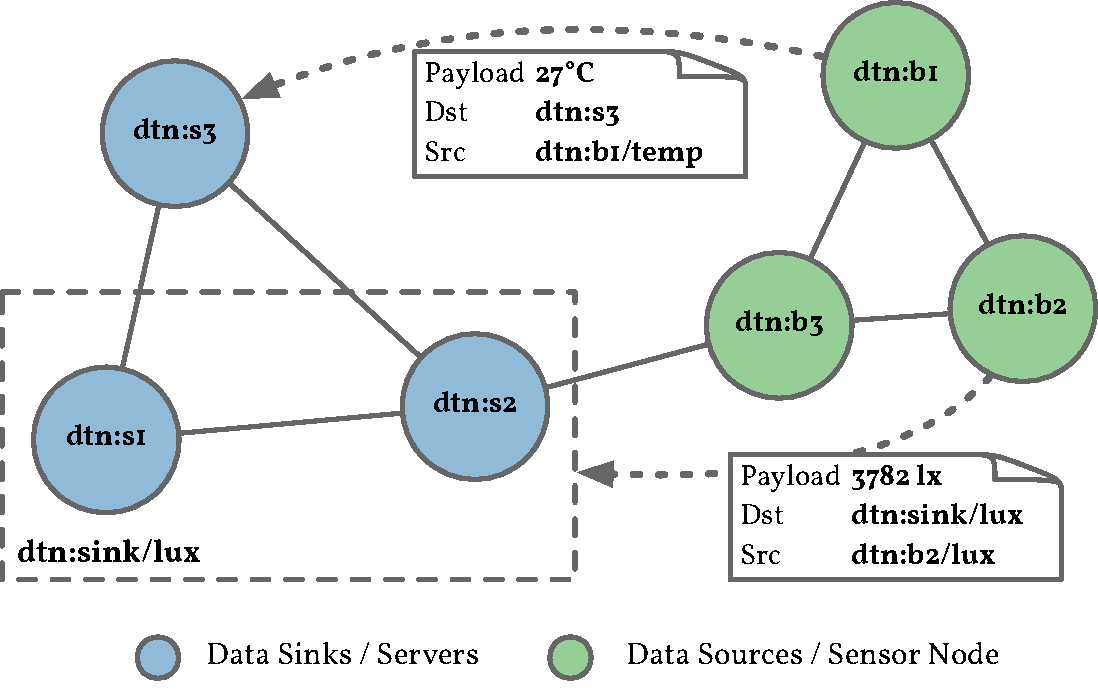
\includegraphics[width=.90\columnwidth]{figs/nodes_endpoints.pdf}
    \caption{Example sensor node scenario with multiple endpoints.}
    \label{penning2019dtn7:fig:nodes_endpoints}
\end{figure}

 
\subsection{Basic Concepts}

\subsubsection{Endpoints.}
\label{penning2019dtn7:ssec:dtn-actors}

In DTN, there are nodes and endpoints.
Nodes exchange bundles according to the store-carry-forward principle. 
Bundles are addressed at endpoints, or more precisely, their characterizing \textit{Endpoint Identifier} (EID), which might not be a currently existing part of the network.
Fig.~\ref{penning2019dtn7:fig:nodes_endpoints} shows an example of a scenario, where sensor nodes produce readings to be consumed by data sinks.
The temperature bundle is addressed directly to \texttt{dtn:s3}, where the lux bundle is headed to \texttt{dtn:sink/lux}, an EID that is handled by two nodes, and thus a multicast. BP7 is endpoint scheme agnostic and supports the null endpoint for anonymous bundles.
In BP version 6, only endpoints are defined, so it is not possible to address dedicated nodes.

\subsubsection{Bundles and Blocks.}

Packets in a DTN consist of multiple \textit{Blocks} to form logical units called \textit{Bundles}.
In Fig.~\ref{penning2019dtn7:fig:bundle-sketch}, an example bundle containing the mandatory Primary Block, and two Canonical Blocks, namely a Hop Count Block and the actual Payload Block, is shown, following the example of Fig.~\ref{penning2019dtn7:fig:nodes_endpoints}.



\begin{figure}[tbph]
    \centering
    \rowcolors{0}{white}{white}
    \resizebox{\textwidth}{!}{
        \begin{tikzpicture}[scale=1.1]
            \begin{umlpackage}[fill=white]{Bundle}
                \umlclass[rectangle split parts=2, fill=white]{Primary Block}{
                    Version: \texttt{7} \\
                    Control Flags: \\
                      \quad \textit{Status requested for reception} \\
                    CRC Type: \textit{None} \\
                    Destination EID: \texttt{dtn:sink/lux} \\
                    Source node EID: \texttt{dtn:b2} \\
                    Report-to EID: \texttt{dtn:b2} \\
                    Creation Timestamp: (\texttt{0}, \texttt{23}) \\
                    Lifetime: \texttt{3600000}
                }{}
                \umlclass[rectangle split parts=2, fill=white, x=4.3, y=0.0]{Hop Count Block}{
                    Type Code: \texttt{9} \\
                    Number: \texttt{2} \\
                    Control Flags: \textit{None} \\
                    CRC Type: \textit{None} \\
                    Data: (\texttt{64}, \texttt{42})
                }{}
                 \umlclass[rectangle split parts=2, fill=white, x=7.65, y=0.0]{Payload Block}{
                    Type Code: \texttt{1} \\
                    Number: \texttt{1} \\
                    Control Flags: \textit{None} \\
                    CRC Type: \textit{None} \\
                    Data: \texttt{0E C6}
                }{}
            \end{umlpackage}
         \end{tikzpicture}
    }
    \caption{A bundle transmitting a lux value from \texttt{dtn:b2} to \texttt{dtn:sink/lux}.}
    \label{penning2019dtn7:fig:bundle-sketch}
\end{figure}


\paragraph{Primary Block.}

Each bundle begins with a (since BP7 immutable) \textit{Primary Block} (see  Fig.~\ref{penning2019dtn7:fig:bundle-sketch}),  containing 
meta-information about the bundle with the following fields:
Version;
Bundle Processing Control Flags to provide information on the bundle, including fragmenting and reporting information;
an optional CRC Checksum (added in BP7 and not available in BP version 6);
Destination EID, Source Node ID and Report-To EID, as  endpoints for administrative records regarding this bundle;
Creation Timestamp, consisting of the actual timestamp and an incrementing sequence number;
Maximum Lifetime of a bundle, expressed in microseconds after creation time;
Fragment Offset and Total Data Length, if fragmented and indicated by the bundle process control flags.

\paragraph{Canonical Block.}
Payload and Extension Blocks in Fig.~\ref{penning2019dtn7:fig:bundle-sketch} are summarized as \textit{Canonical Blocks}. 
These contain a payload in addition to a few block-specific characteristics.
A Canonical Block consists of a Type Code to identify the kind of block, Number to address the specific block, Control Flags and Data. 
% The most important canonical blocks are discussed below. 

The actual payload of the bundle is located in the Payload Block at the end of each bundle.
In addition to sending user data from application programs, status information is also sent within bundles, called Administrative Records, automatically created and sent by DTN software as a response to a previous bundle. 
Extension Blocks are Canonical Blocks containing further information relevant for a DTN router depending on its configuration.
In contrast to BP version 6, the BP7 specification defines the Previous Node Block, Bundle Age Block, and Hop Count Block, and allows user-defined blocks to be added.



\subsection{Node Components}

\subsubsection{Bundle Protocol Agent.}
The \textit{Bundle Protocol Agent} (BPA) offers BP and DTN specific services.
It executes procedures of the BP.
For example, communication between Application Agent and Convergence Layer Adapter (see below) is managed.
The BPA also constructs bundles for the Application Agent.

\subsubsection{Application Agent.}
The interface between the BPA and an application is defined as an \textit{Application Agent} (AA).
A generic AA needs the ability to receive incoming bundles and compose outbound bundles for user applications and services.
Furthermore, an EID must be assigned for local bundle delivery.

\subsubsection{Convergence Layers.}
Bundles are exchanged over connections between nodes of different types and characteristics, and connections are unidirectional or bidirectional, or vary in transmission speed and bandwidth.
Depending on the connection technology used, more or less complex protocols are required for delivery, called \textit{Convergence Layer (CL) Protocols} (CLP).
A \textit{Convergence Layer Adapter} (CLA) is an implementation of a CLP.
There are two CLPs defined by the IETF DTN group to exchange bundles over a TCP connection, the bidirectional TCP Convergence Layer Protocol (TCPCL)~\cite{dtn_tcp} and the unidirectional Minimal TCP Convergence Layer Protocol (MTCP)~\cite{dtn_mtcp}.
In addition to transport layer CLs, there are approaches based on other technologies, e.g., DTN2 defining a Bluetooth and a serial CL, or IRB-DTN featuring an e-mail CL.
